\documentclass[12pt]{article}
\usepackage{graphicx}

\begin{document}
    {\Large \textbf{Doppler Effect and Photoelectric Effect} \par}

    \section*{Definitions}
    \textbf{Doppler effect}: Change in wavelength (or frequency) of light coming from an object because
    it is in motion.

    \begin{figure}[h]
        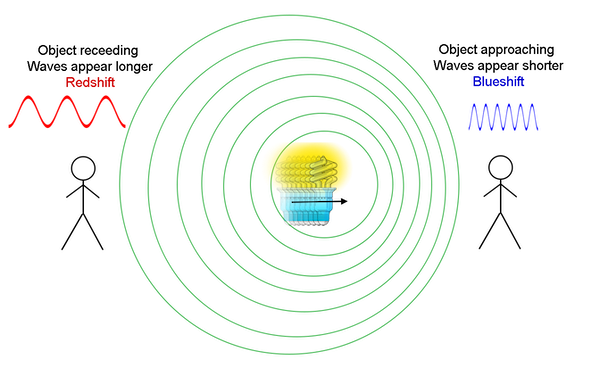
\includegraphics[scale = 0.5]{doppler_shift_light.png}
    \end{figure}

    \noindent \textbf{Photoelectric effect}: Electron may be excited to a higher (discrete) energy level from the ground state 
    (potentially by a photon) and when it drops down energy levels it emits a photon with the same energy that it lost.

    \begin{figure}[ht]
        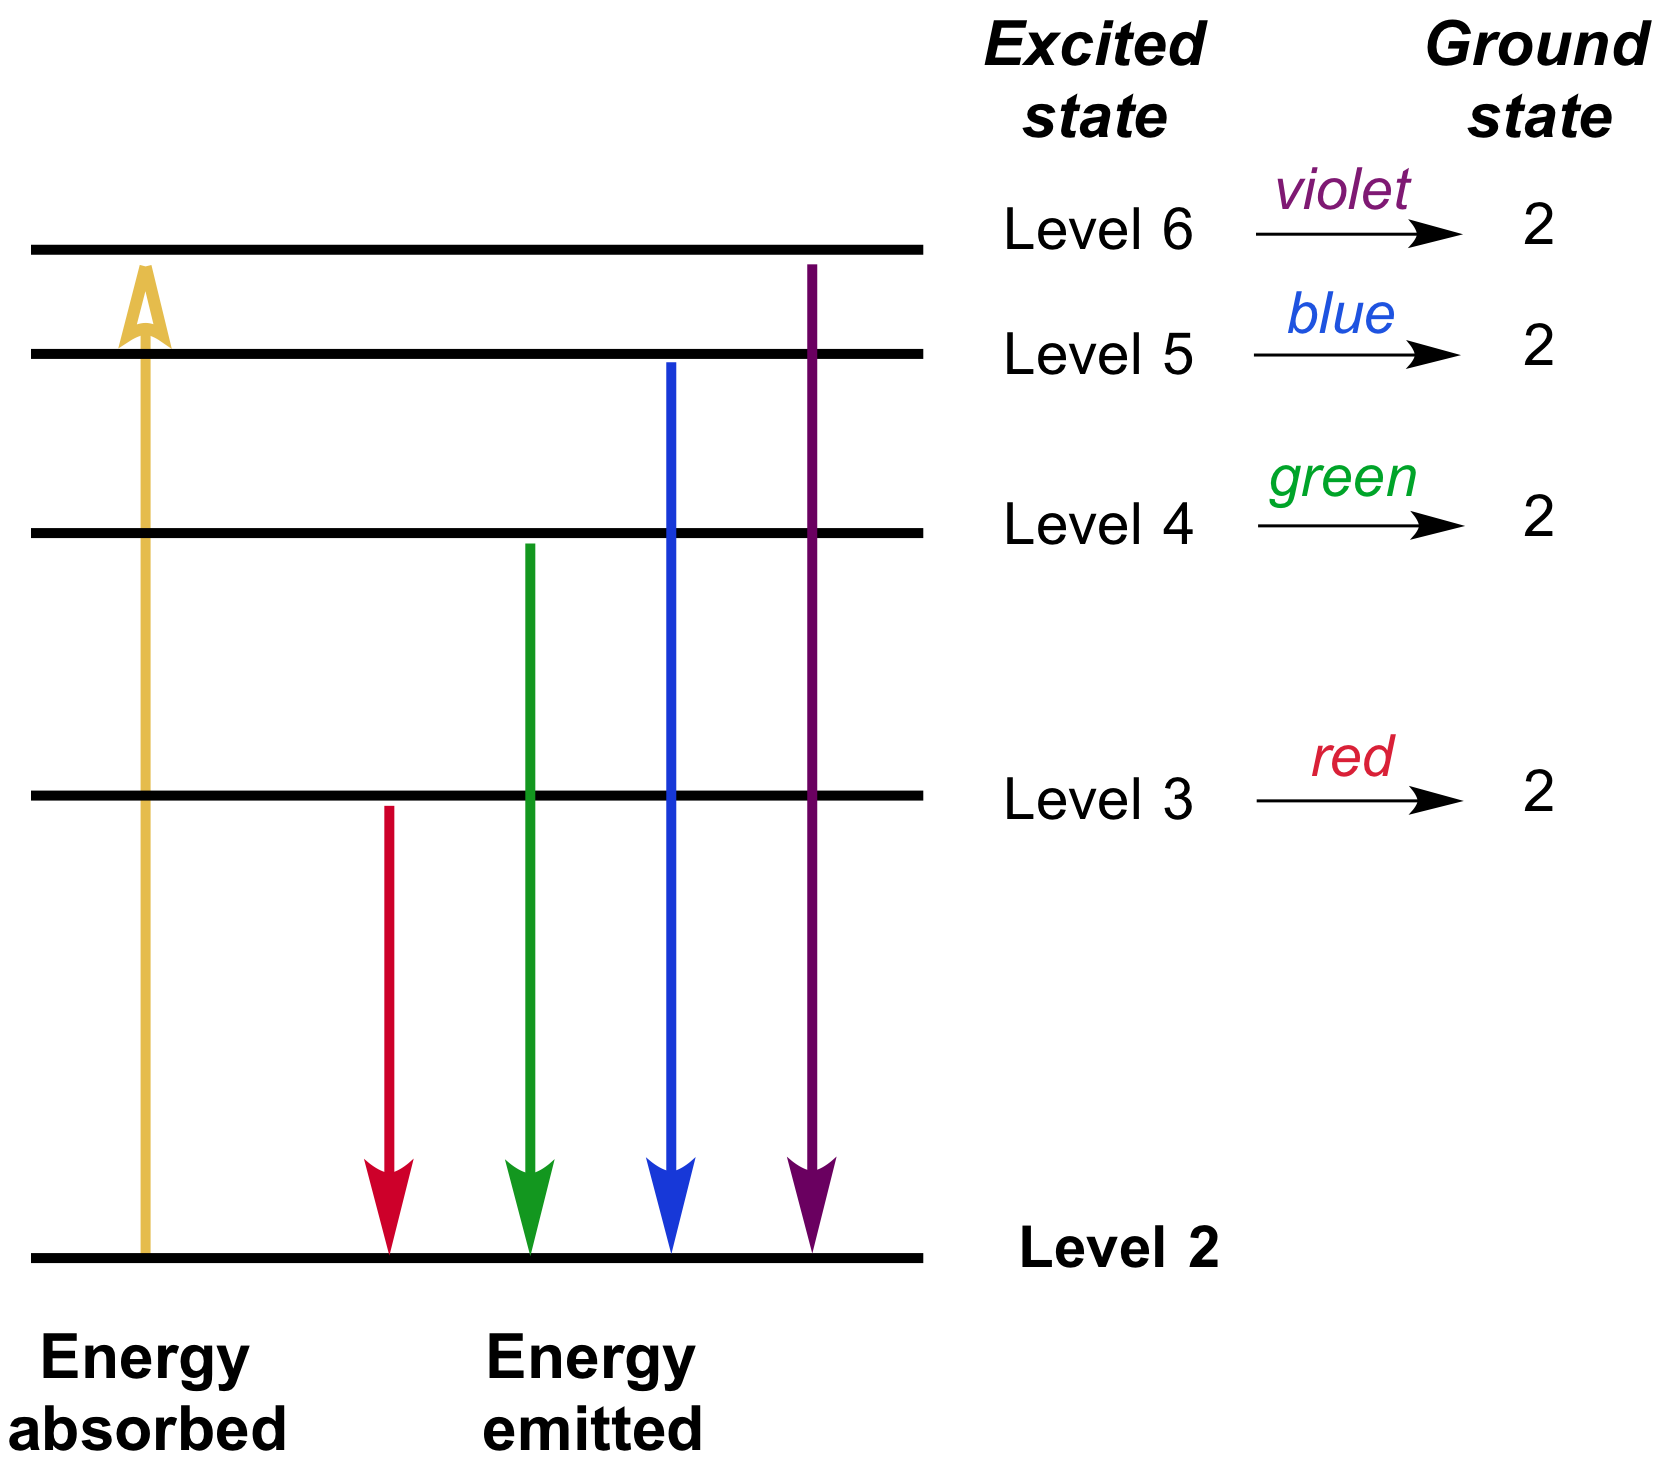
\includegraphics[scale = 0.5]{b8cb777559d81c6a6640187549bcd3907ebf0573.png}
    \end{figure}

    \section*{Formulas}
    \begin{enumerate}
        \item $z = \frac{\Delta \lambda}{\lambda} \approx \frac{\Delta f}{f} \approx \frac{v}{c}$
        \item $v=H_{0}d$
        \item $v = f\lambda$
        \item $E=hf$
        \item $hf = \phi + \frac{1}{2}mv^2$
    \end{enumerate}

    %why isnt the night sky super bright from all the stars in the universe? A lot of stars are super far away,
    %so far that they actually redshift to infrared light
    %age of universe and ultimate fate
    %spectra lines from absorbtion of photon, leading into photoelectric effect

    \section*{Age of the universe (simplified)}
    In the formulas above, $H_{0}$ is the Hubble's constant. Why is this constant so important? Recall that $v=d/t$ (speed = distance/time).
    Subbing in $v = H_{0}d$ and rearranging you get $t=1/H_{0}$. This allows us to calculate the age of the universe. \newline
    $H_{0}$ (measures the rate of expansion of the universe) seems to be accelerating which means the universe may expand 
    forever at an increasing rate. This is known as the Big Freeze or Big Rip theory (open universe). On the other hand, some people believe the rate will
    slow down and the universe will start contracting back into a singularity. This is know as the Big Crunch theory (closed universe). \newline
    Some evidence for dark matter comes from the fact that certain galaxies behave as if they have much more mass in them. Other evidence
    is via gravitational lensing.

    \begin{figure}[h]
        \centering
        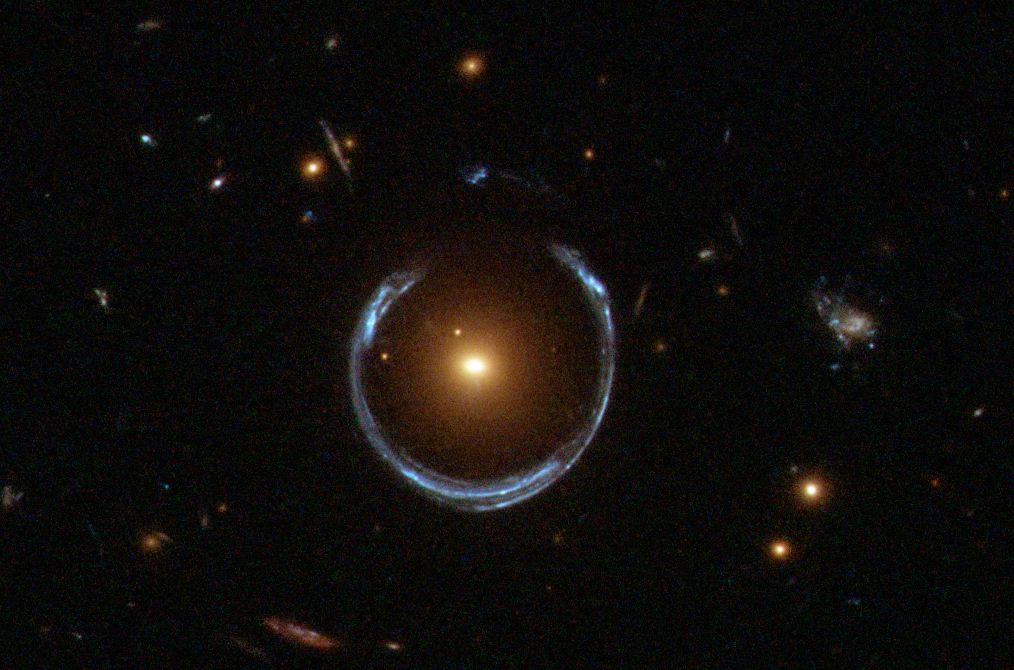
\includegraphics[scale = 0.2]{A_Horseshoe_Einstein_Ring_from_Hubble.jpg}
        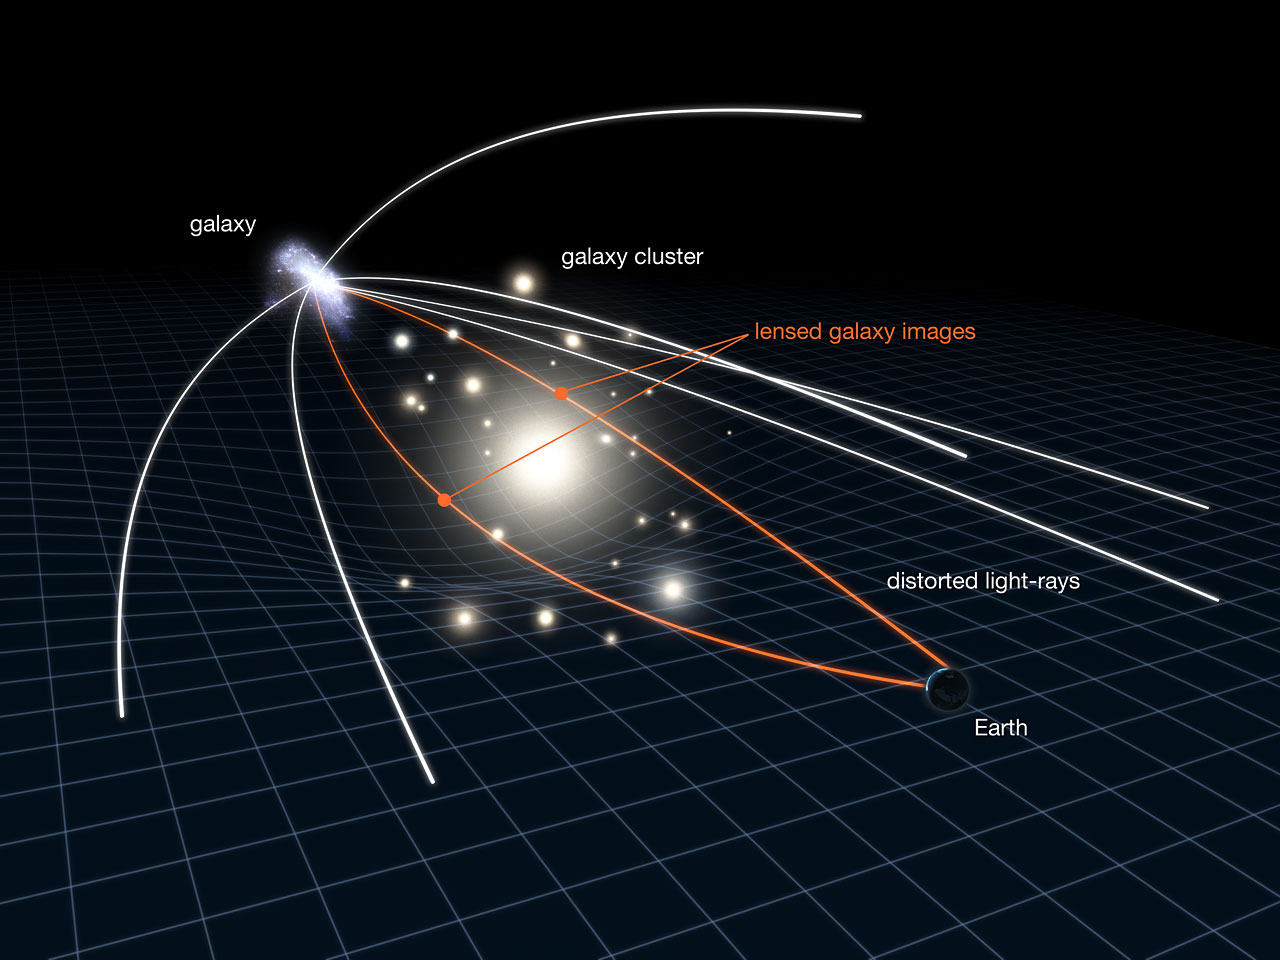
\includegraphics[scale = 0.12]{heic1106c.jpg}
    \end{figure}

    \section*{Spectra Lines}
    Spectra lines are like the fingerprints of an element. They are the bits of the spectrum that are
    absorbed by the element when photons pass through it. These frequencies correspond to the differences
    between the discrete energy levels of the element.

    \begin{figure}[h]
        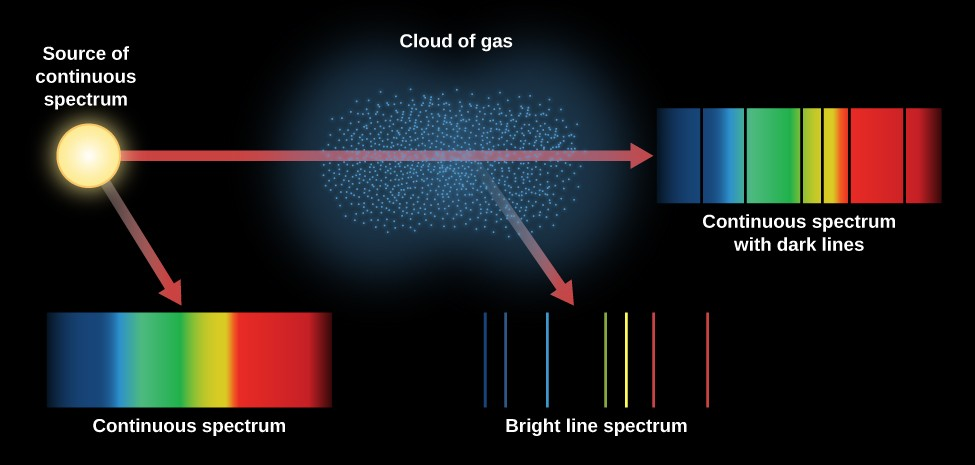
\includegraphics[width = \linewidth]{OSC_Astro_05_05_TSpectra.jpg}
    \end{figure}

    \section*{Photoelectric Effect}
    The photoelectric effect provides some evidence for light being a particle as only specific energies of
    light can excite electrons instead. If light was a wave it would slowly transfer energy to electrons
    and they would be excited given enough time from light of any wavelength or frequency. (Recall that the
    double slit experiment)

    \section*{Work Function and Threshold Frequency}
    The work function, $\phi$, is the minimum amount of energy required to remove an electron from the atom.
    The electron that is removed is called a photoelectron.
    Threshold frequency is the corresponding to the work function. So using $E = hf$ we see the
    threshold frequency is $\phi/h$.


\end{document}